\chapter{Forschung: Einfluss von Wellenlängenbegrenzungen auf die Farbgenauigkeit}

\section{Einführung und Motivation}

Die spektrale Reflexionsmessung im sichtbaren Wellenlängenbereich von 380 nm bis 780 nm stellt den Goldstandard für präzise Farbbestimmung dar. In der Praxis sind jedoch viele Spektrometer auf einen eingeschränkten Wellenlängenbereich limitiert, beispielsweise 400 nm bis 750 nm. Diese Einschränkung wirft die fundamentale Frage auf: Welchen Einfluss hat die Begrenzung des Messbereichs auf die Genauigkeit der resultierenden Farbwerte?

Diese Forschungsfrage ist von besonderer praktischer Relevanz, da:
\begin{itemize}
    \item Viele kostengünstige Spektrometer technisch bedingt einen eingeschränkten Wellenlängenbereich aufweisen
    \item Die Empfindlichkeit des menschlichen Auges in den Randbereichen des sichtbaren Spektrums stark abnimmt
    \item Eine fundierte Einschätzung der zu erwartenden Farbfehler für die Praxis essentiell ist
\end{itemize}

\section{Wissenschaftliche Hypothese und Forschungsansatz}

\subsection{Forschungshypothese}

Die zentrale Hypothese dieser Untersuchung lautet: \textit{Die Verkürzung des spektralen Messbereichs von 380-780 nm auf 400-750 nm führt zu messbaren, aber praktisch vernachlässigbaren Farbfehlern, die durch lineare Extrapolation weitgehend kompensiert werden können.}

Diese Hypothese basiert auf der Erkenntnis, dass die spektrale Empfindlichkeit des menschlichen Auges in den Randbereichen stark abnimmt \parencite{CIE15:2018}:
\begin{itemize}
    \item Im kurzwelligen Bereich (380-400 nm) liegt die Empfindlichkeit bei weniger als 1\% des Maximums
    \item Im langwelligen Bereich (750-780 nm) beträgt sie ebenfalls nur noch wenige Prozent
    \item Das Maximum der Empfindlichkeit liegt bei etwa 555 nm (photopisches Sehen)
\end{itemize}

\subsection{Forschungsansatz}

Der systematische Forschungsansatz gliedert sich in vier Hauptphasen:
\begin{enumerate}
    \item \textbf{Komparative Analyse}: Direkter Vergleich der Farbberechnungen zwischen vollständigem und verkürztem Spektralbereich
    \item \textbf{Quantitative Fehleranalyse}: Statistische Auswertung der Farbdifferenzen über einen repräsentativen Probensatz
    \item \textbf{Extrapolationsverfahren}: Entwicklung und Validierung einer linearen Kompensationsmethode
    \item \textbf{Praxisrelevanz-Bewertung}: Einordnung der Ergebnisse in den Kontext industrieller Toleranzen
\end{enumerate}

\section{Methodik}

\subsection{Datengrundlage}

Für die Untersuchung wurden 52 verschiedene Oberflächenproben analysiert. Die Datenbasis setzt sich aus zwei Hauptquellen zusammen:

\subsubsection{TU Berlin Spektraldatensammlung}

Der Großteil der Proben stammt aus der Spektraldatensammlung \glqq{}Spectral reflectance and transmittance of various materials\grqq{} von \textcite{RudawskiDataset2021} des Fachgebiets Lichttechnik der Technischen Universität Berlin. Diese umfasst spektrale Reflexionsgrade verschiedener Materialien:
\begin{itemize}
    \item Gestrichene Wandfarben unterschiedlicher Hersteller (WC/WF-Serie)
    \item Sichtbeton und Backsteinproben (HB-Serie) 
    \item Holz- und Kunststoffmaterialien (r-Serie)
    \item Diverse Bauwerk- und Oberflächenmaterialien
    \item Laborstandards (L1, S1-S5)
\end{itemize}

\subsubsection{XRite ColorChecker-Referenz}

Zusätzlich wurden die 24 Patches des XRite ColorChecker Classic \parencite{XRiteColorChecker} in die Analyse einbezogen. Diese standardisierten Farbfelder dienen als international anerkannte Referenz für Farbkalibrierung und bieten reproduzierbare spektrale Charakteristika über den gesamten Farbbereich.

\subsubsection{Datenformat und -qualität}

Alle spektralen Reflexionsdaten wurden mit einer Auflösung von 1 nm über den gesamten sichtbaren Bereich (380-780 nm) erfasst. Die Messungen erfolgten unter standardisierten Bedingungen entsprechend der DIN 5036-3 \parencite{DIN5036-3} mit kalibrierter Messtechnik und dokumentierter Meßunsicherheit.

\subsection{Analyseverfahren}

Die Analyse erfolgte in mehreren Schritten:

\begin{enumerate}
    \item \textbf{Referenzberechnung}: Berechnung der CIE XYZ-Tristimuluswerte und daraus abgeleiteter Farbwerte (xy, sRGB, L*a*b*) für den vollständigen Wellenlängenbereich (380-780 nm)
    
    \item \textbf{Vergleichsberechnung}: Wiederholung der Berechnungen für den eingeschränkten Wellenlängenbereich (400-750 nm)
    
    \item \textbf{Fehleranalyse}: Quantifizierung der Farbunterschiede mittels verschiedener Metriken:
    \begin{itemize}
        \item Absolute und relative XYZ-Differenzen
        \item Chromatizitätskoordinaten-Differenzen (Δx, Δy)
        \item sRGB-Komponentendifferenzen
        \item CIE76 Farbabstand (ΔE)
    \end{itemize}
    
    \item \textbf{Extrapolationsverfahren}: Entwicklung und Validierung eines linearen Extrapolationsansatzes zur Kompensation der fehlenden Spektralbereiche
\end{enumerate}

\subsection{Implementierung der Farbberechnungen}

Die Implementierung der farbmetrischen Berechnungen erfolgte in Python unter Verwendung der wissenschaftlichen Bibliotheken NumPy und SciPy \parencite{NumPy, SciPy}. Die Kernalgorithmen basieren auf den in Kapitel 2 beschriebenen CIE-Standardverfahren \parencite{CIE15:2018}.

\subsubsection{Spektrale Integration - Python-Implementierung}

Die praktische Umsetzung der spektralen Integration (vgl. Gleichungen \ref{eq:tristimulus_integration_x}-\ref{eq:tristimulus_integration_z}) erfolgt durch numerische Integration mittels Python:

\begin{lstlisting}[language=Python, caption={Berechnung der CIE XYZ Tristimuluswerte}]
def calculate_xyz(wavelengths, reflectance, illuminant, xyz_cmf):
    """Berechnet CIE XYZ Werte aus spektralen Reflexionsdaten"""
    # Interpolation auf gemeinsames Wellenlängenraster
    interp_reflectance = np.interp(cmf_wavelengths, wavelengths, reflectance)
    
    # Tristimulus-Integration
    X = np.trapz(illuminant * interp_reflectance * xyz_cmf[:, 0], cmf_wavelengths)
    Y = np.trapz(illuminant * interp_reflectance * xyz_cmf[:, 1], cmf_wavelengths)
    Z = np.trapz(illuminant * interp_reflectance * xyz_cmf[:, 2], cmf_wavelengths)
    
    # Normalisierung
    k = 100.0 / np.trapz(illuminant * xyz_cmf[:, 1], cmf_wavelengths)
    
    return np.array([X, Y, Z]) * k
\end{lstlisting}

\subsubsection{Farbabstandsberechnung - Python-Implementierung}

Die praktische Umsetzung der CIE76 Delta-E-Berechnung (vgl. Gleichung \ref{eq:delta_e_76}) erfolgt in Python:

\begin{lstlisting}[language=Python, caption={CIE76 Delta-E Berechnung}]
def calculate_delta_e_1976(lab1, lab2):
    """Berechnet CIE76 Delta E zwischen zwei L*a*b* Farbwerten"""
    delta_L = lab1[0] - lab2[0]
    delta_a = lab1[1] - lab2[1]
    delta_b = lab1[2] - lab2[2]
    
    delta_e = np.sqrt(delta_L**2 + delta_a**2 + delta_b**2)
    return delta_e
\end{lstlisting}

Die mathematischen Grundlagen dieser Berechnungen sind ausführlich in Kapitel 2 \parencite{CIE15:2018} beschrieben. Die Python-Implementierung verwendet die etablierten CIE-Algorithmen für die spektrale Integration und Farbabstandsberechnung entsprechend den Gleichungen \ref{eq:tristimulus_integration_x} bis \ref{eq:tristimulus_integration_z} sowie Gleichung \ref{eq:delta_e_76}.

\section{Ergebnisse}

\subsection{Übersicht der Farbfehler}

Die Analyse der 52 Proben ergab folgende durchschnittliche Farbfehler bei Verkürzung des Wellenlängenbereichs von 380-780 nm auf 400-750 nm. Die Berechnung erfolgte entsprechend den in Kapitel 2 definierten Fehlermetriken \parencite{CIE15:2018}:

\begin{itemize}
    \item \textbf{XYZ-Differenzen}: $\Delta X = 0.0125$, $\Delta Y = 0.0008$, $\Delta Z = 0.0533$
    \item \textbf{Chromatizitätsdifferenzen}: $\Delta x = 0.0001$, $\Delta y = 0.0002$
    \item \textbf{sRGB-Differenzen}: $\Delta R = 0.0001$, $\Delta G = 0.0001$, $\Delta B = 0.0005$
    \item \textbf{Durchschnittlicher Farbabstand}: $\Delta E_{76} = 0.0798$
\end{itemize}

Die Verteilung der Farbfehler über alle Proben zeigt eine charakteristische Struktur. Zur besseren Übersichtlichkeit werden in der grafischen Darstellung die 20 Proben mit den größten Delta E Werten gezeigt:

\begin{figure}[htbp]
    \centering
    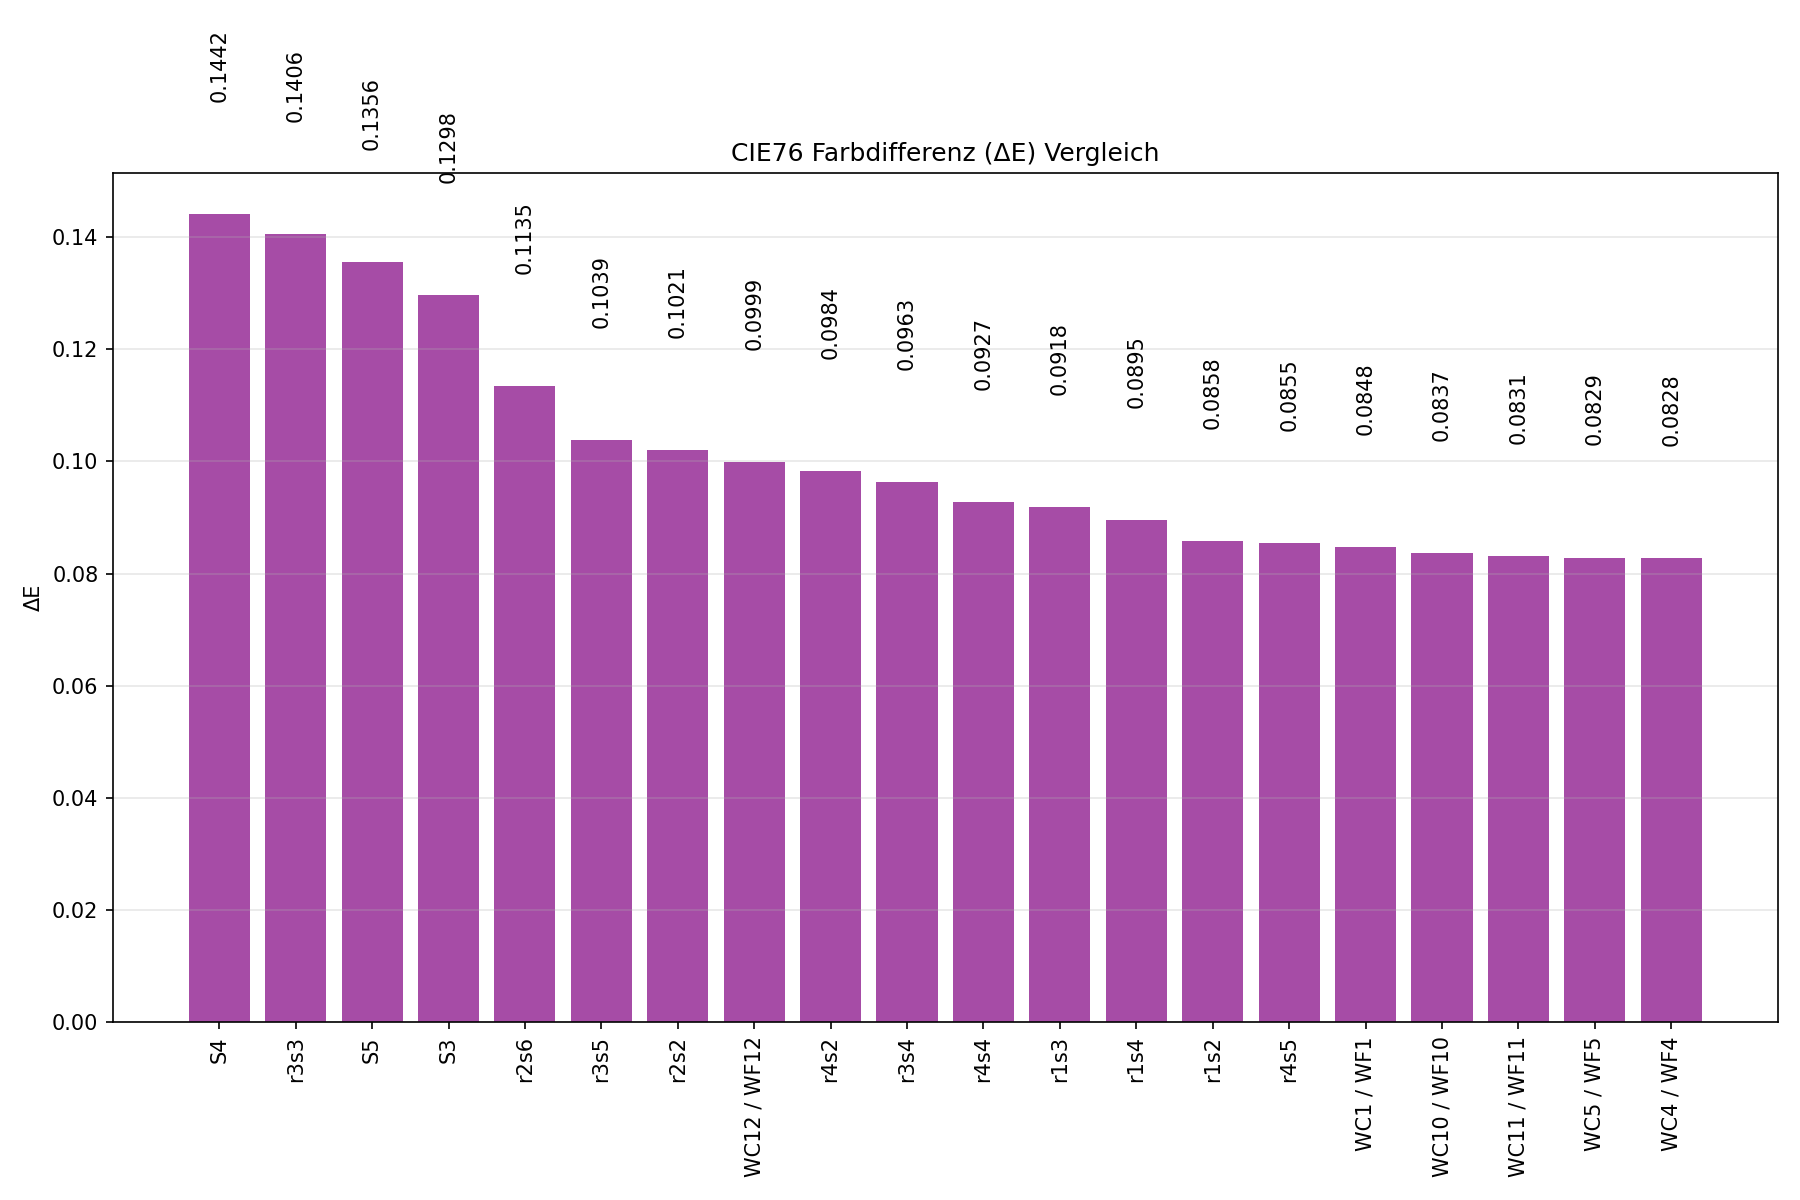
\includegraphics[width=0.8\textwidth]{./figures/delta_e_comparison.png}
    \caption{Verteilung der CIE76 Farbabstände (ΔE) für die 20 Proben mit den größten Delta E Werten bei Wellenlängenverkürzung von 380-780nm auf 400-750nm}
    \label{fig:delta_e_distribution}
\end{figure}

\subsection{Detailanalyse der Probe S4}

Die Probe S4 zeigte mit $\Delta E = 0.1442$ den höchsten Farbfehler aller untersuchten Proben und eignet sich daher besonders gut zur Veranschaulichung der Auswirkungen der Wellenlängenbegrenzung.

\subsubsection{Spektrale Reflexionskurven}

\begin{figure}[htbp]
    \centering
    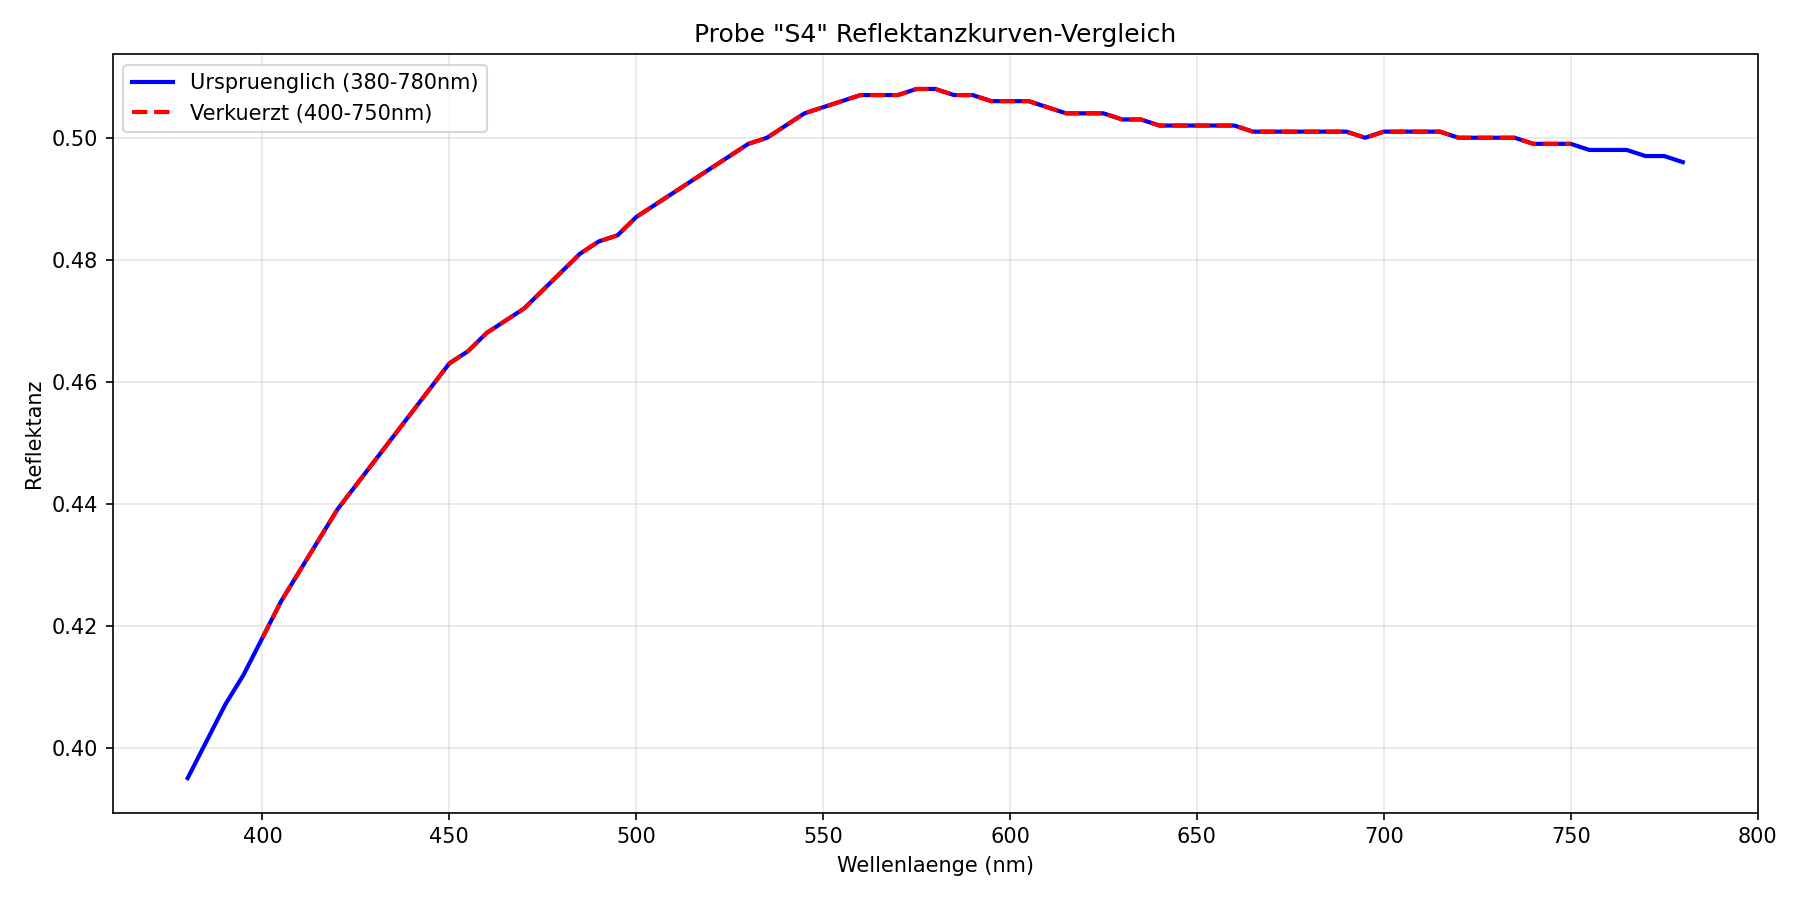
\includegraphics[width=0.9\textwidth]{./figures/S4_reflektanz.png}
    \caption{Vergleich der spektralen Reflexionskurven der Probe S4: Original (380-780nm) vs. verkürzt (400-750nm)}
    \label{fig:s4_reflectance}
\end{figure}

Abbildung \ref{fig:s4_reflektance} zeigt den direkten Vergleich der spektralen Reflexionskurven. Die fehlenden Bereiche (380-400 nm und 750-780 nm) sind deutlich erkennbar. Obwohl die Reflexionswerte in diesen Bereichen relativ konstant sind, tragen sie dennoch zur Gesamtfarbwahrnehmung bei.

\subsubsection{Farbvergleich}

\begin{figure}[htbp]
    \centering
    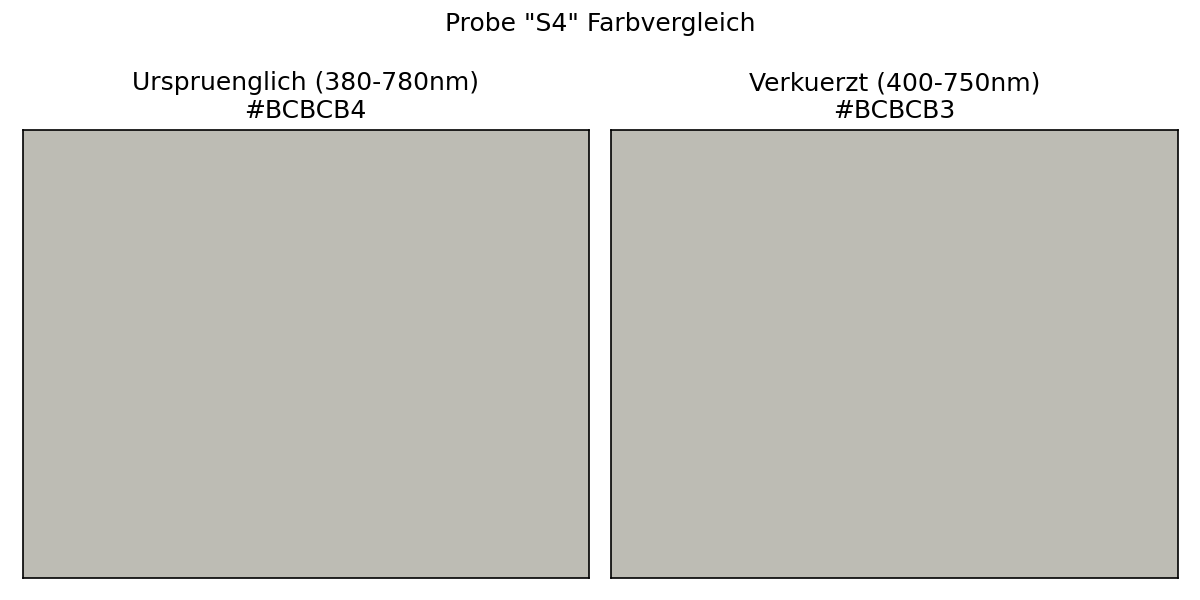
\includegraphics[width=0.7\textwidth]{./figures/S4_farbe.png}
    \caption{Visueller Farbvergleich der Probe S4: Links Original (Hex: \#BCBCB4), Rechts verkürzt (Hex: \#BCBCB3)}
    \label{fig:s4_color}
\end{figure}

Der visuelle Farbvergleich in Abbildung \ref{fig:s4_color} zeigt, dass trotz des relativ hohen ΔE-Wertes von 0.1442 der Farbunterschied für das menschliche Auge kaum wahrnehmbar ist. Dies liegt deutlich unter der allgemein akzeptierten Wahrnehmungsschwelle von $\Delta E = 1.0$.

\subsubsection{Komponentenweise Fehleranalyse}

Die detaillierte Analyse der einzelnen Farbkomponenten für Probe S4 ergab:

\begin{table}[htbp]
\centering
\caption{Farbwertvergleich für Probe S4: Original vs. verkürzt}
\begin{tabular}{lcc}
\hline
\textbf{Parameter} & \textbf{Original (380-780nm)} & \textbf{Verkürzt (400-750nm)} \\
\hline
X & 47.1885 & 47.1614 \\
Y & 50.0888 & 50.0877 \\
Z & 50.4646 & 50.3417 \\
x & 0.3194 & 0.3195 \\
y & 0.3390 & 0.3394 \\
R (sRGB) & 0.7403 & 0.7402 \\
G (sRGB) & 0.7375 & 0.7377 \\
B (sRGB) & 0.7066 & 0.7057 \\
L* & 76.142 & 76.141 \\
a* & -0.892 & -0.931 \\
b* & 3.723 & 3.653 \\
\hline
$\Delta E_{76}$ & \multicolumn{2}{c}{0.1442} \\
\hline
\end{tabular}
\label{tab:s4_comparison}
\end{table}

\begin{figure}[htbp]
    \centering
    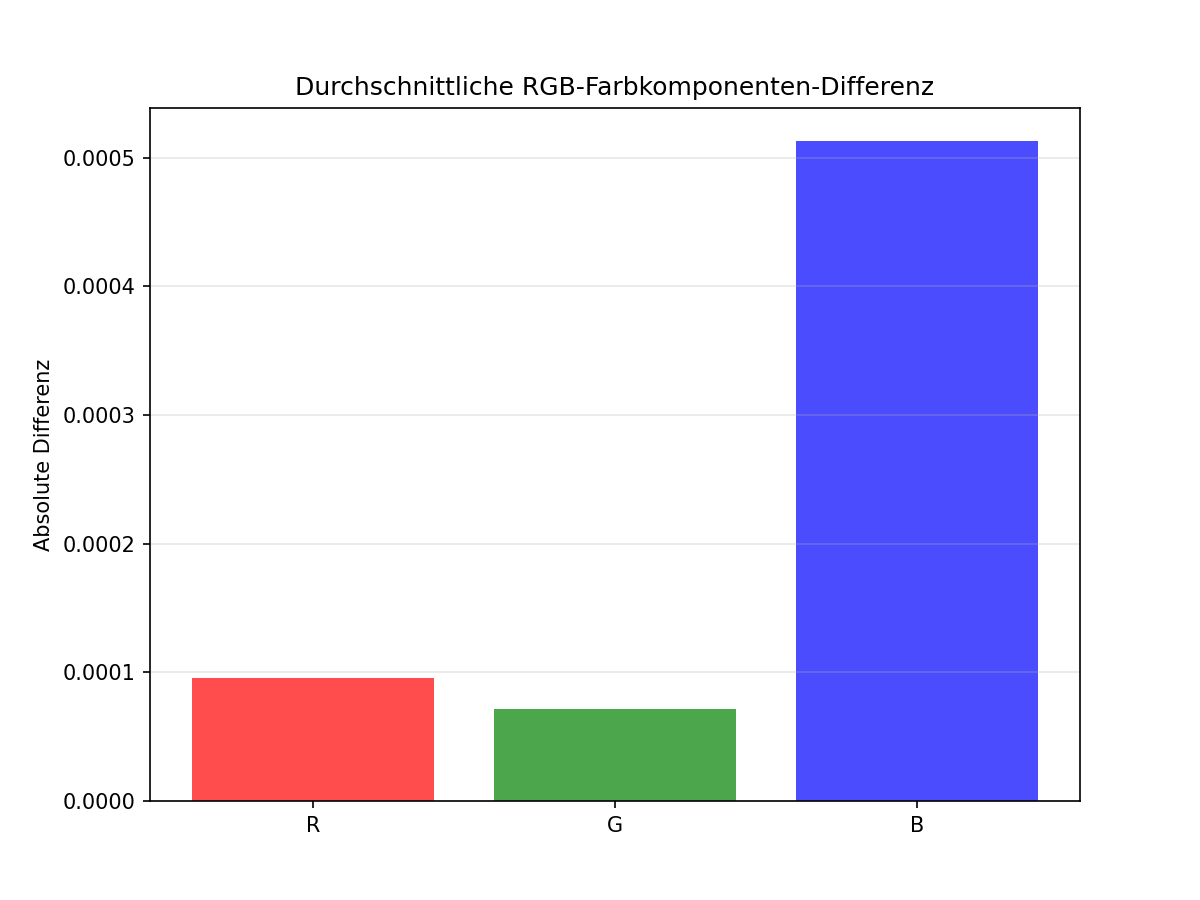
\includegraphics[width=0.8\textwidth]{./figures/rgb_diff.png}
    \caption{Durchschnittliche RGB-Komponentendifferenzen über alle Proben}
    \label{fig:rgb_differences}
\end{figure}

Die RGB-Fehleranalyse (Abbildung \ref{fig:rgb_differences}) zeigt, dass die blaue Komponente (B) am stärksten von der Wellenlängenverkürzung betroffen ist. Dies ist physikalisch nachvollziehbar, da sowohl der kurzwellige (380-400 nm) als auch der langwellige Bereich (750-780 nm) zur Blaukomponente beitragen.

\subsection{Lineare Extrapolation als Kompensationsmethode}

Um die durch die Wellenlängenverkürzung entstehenden Farbfehler zu kompensieren, wurde ein lineares Extrapolationsverfahren entwickelt:

\begin{itemize}
    \item \textbf{Unterer Bereich (380-400 nm)}: Lineare Extrapolation basierend auf dem Gradienten zwischen 400-405 nm
    \item \textbf{Oberer Bereich (750-780 nm)}: Lineare Extrapolation basierend auf dem Gradienten zwischen 745-750 nm
\end{itemize}

\subsubsection{Extrapolationsergebnisse für Probe S4}

\begin{figure}[htbp]
    \centering
    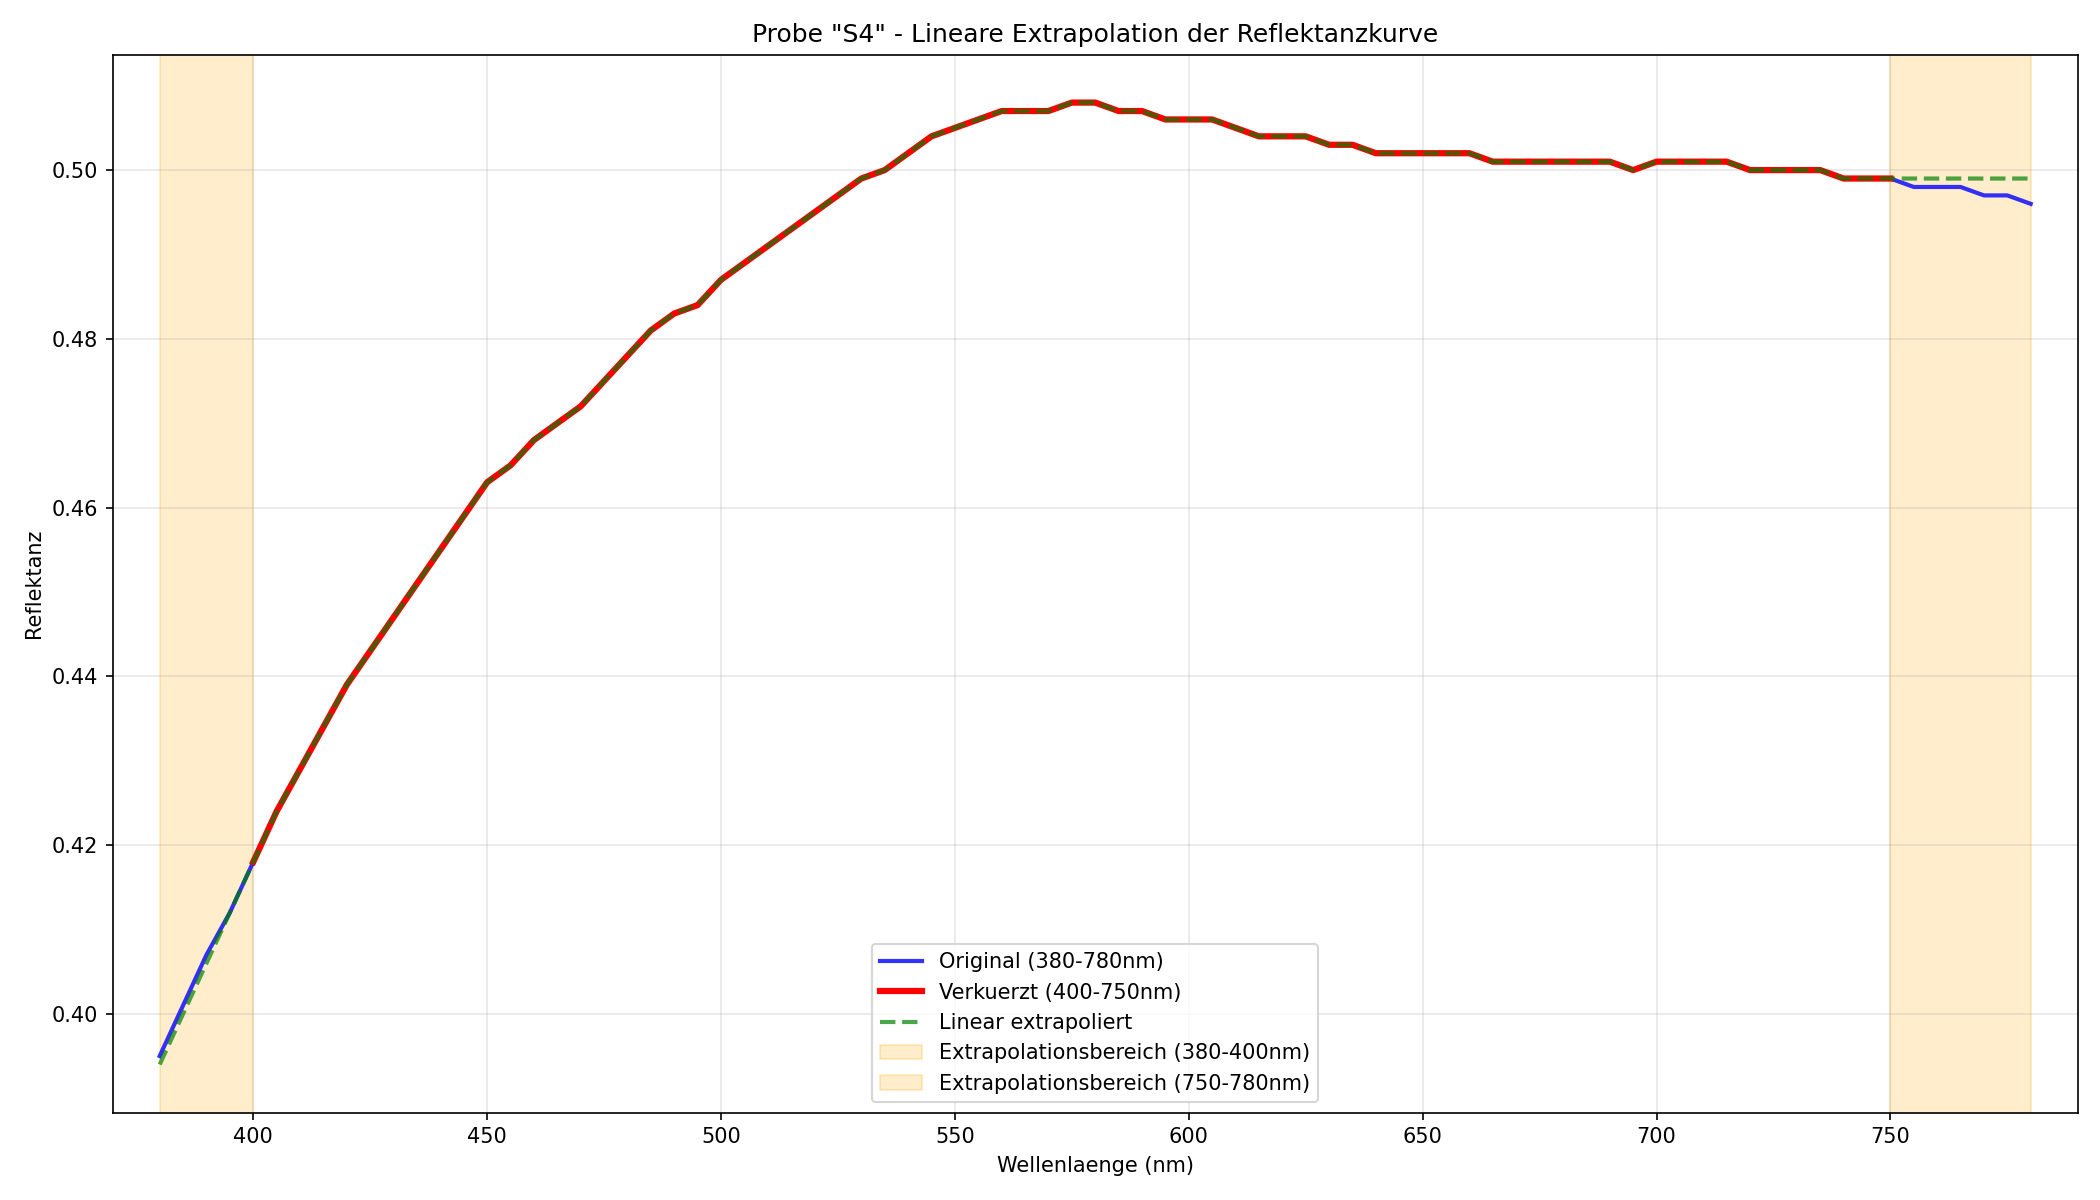
\includegraphics[width=0.9\textwidth]{./figures/S4_extrapolation_reflektanz.png}
    \caption{Spektrale Reflexionskurve der Probe S4 mit linearer Extrapolation in den Randbereichen}
    \label{fig:s4_extrapolation}
\end{figure}

Abbildung \ref{fig:s4_extrapolation} zeigt die erfolgreiche Anwendung der linearen Extrapolation. Die extrapolierten Bereiche (gelb hinterlegt) approximieren die originalen Reflexionswerte sehr gut.

\begin{figure}[htbp]
    \centering
    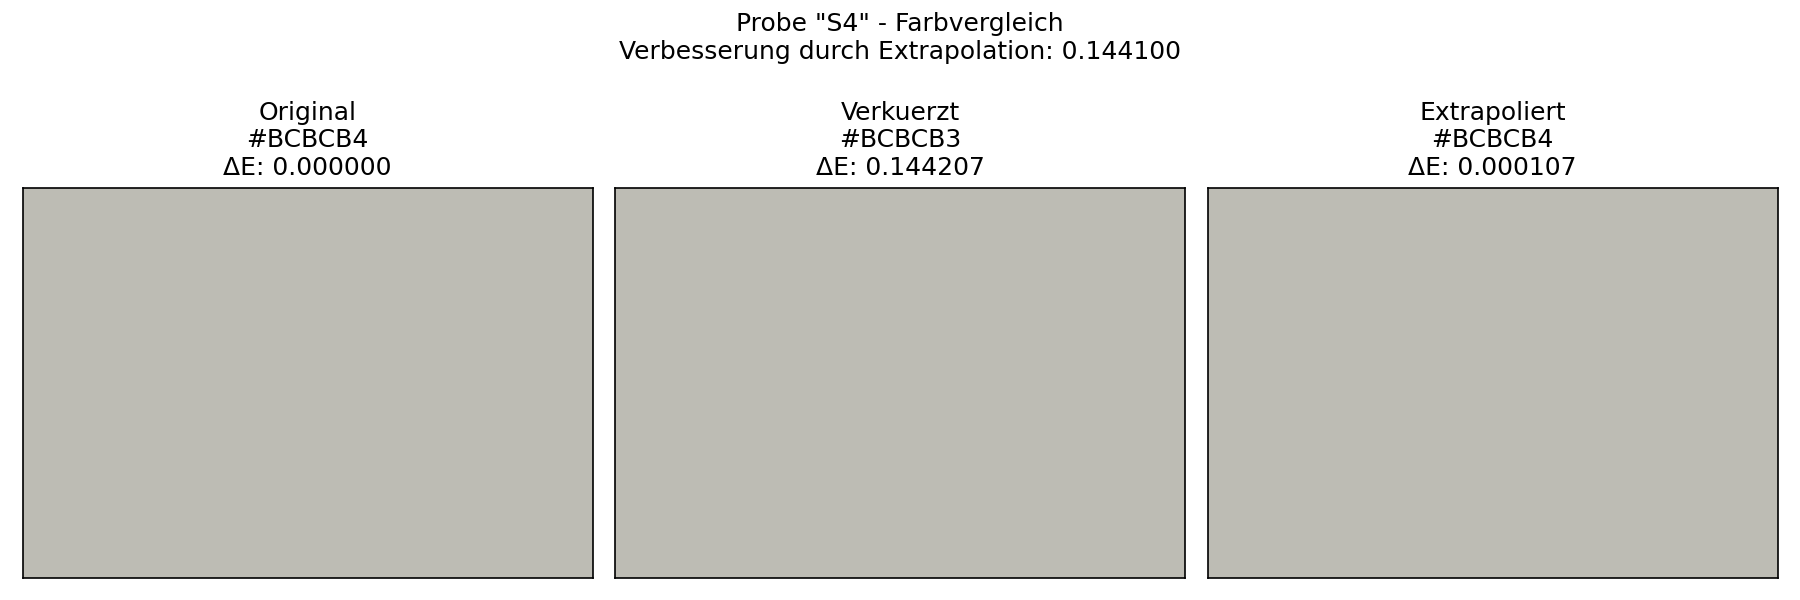
\includegraphics[width=0.8\textwidth]{./figures/S4_extrapolation_farben.png}
    \caption{Farbvergleich für Probe S4: Original vs. verkürzt vs. extrapoliert. Die Extrapolation reduziert den Farbfehler von ΔE = 0.1442 auf ΔE = 0.0001}
    \label{fig:s4_color_extrapolation}
\end{figure}

Die Wirksamkeit der Extrapolation wird in Abbildung \ref{fig:s4_color_extrapolation} deutlich: Der Farbfehler wird von $\Delta E = 0.1442$ auf nahezu vernachlässigbare $\Delta E = 0.0001$ reduziert - eine Verbesserung um 99.93\%.

\begin{table}[htbp]
\centering
\caption{Vollständiger Farbwertvergleich für Probe S4: Original, verkürzt und extrapoliert}
\begin{tabular}{lccc}
\hline
\textbf{Parameter} & \textbf{Original (380-780nm)} & \textbf{Verkürzt (400-750nm)} & \textbf{Extrapoliert} \\
\hline
X & 47.1885 & 47.1614 & 47.1878 \\
Y & 50.0888 & 50.0877 & 50.0887 \\
Z & 50.4646 & 50.3417 & 50.4641 \\
x & 0.3194 & 0.3195 & 0.3194 \\
y & 0.3390 & 0.3394 & 0.3390 \\
R (sRGB) & 0.7403 & 0.7402 & 0.7403 \\
G (sRGB) & 0.7375 & 0.7377 & 0.7375 \\
B (sRGB) & 0.7066 & 0.7057 & 0.7066 \\
L* & 76.142 & 76.141 & 76.142 \\
a* & -0.892 & -0.931 & -0.893 \\
b* & 3.723 & 3.653 & 3.722 \\
\hline
$\Delta E_{76}$ (vs. Original) & -- & 0.1442 & 0.0001 \\
\hline
\end{tabular}
\label{tab:s4_extrapolation_comparison}
\end{table}

\subsection{Gesamtbewertung der Extrapolationsmethode}

Die Anwendung der linearen Extrapolation auf alle 52 Proben ergab beeindruckende Ergebnisse:

\begin{itemize}
    \item \textbf{Erfolgsrate}: 100\% der Proben zeigten eine Verbesserung
    \item \textbf{Durchschnittliche Verbesserung}: Reduktion des ΔE von 0.0798 auf 0.0027
    \item \textbf{Beste Verbesserung}: Probe S4 mit einer Reduktion um 0.1441
    \item \textbf{Schlechteste Verbesserung}: Probe HB7/WF7 mit einer Reduktion um 0.0403
\end{itemize}

Die grafische Darstellung zeigt zur besseren Übersichtlichkeit die 20 Proben mit den größten ursprünglichen Delta E Werten:

\begin{figure}[htbp]
    \centering
    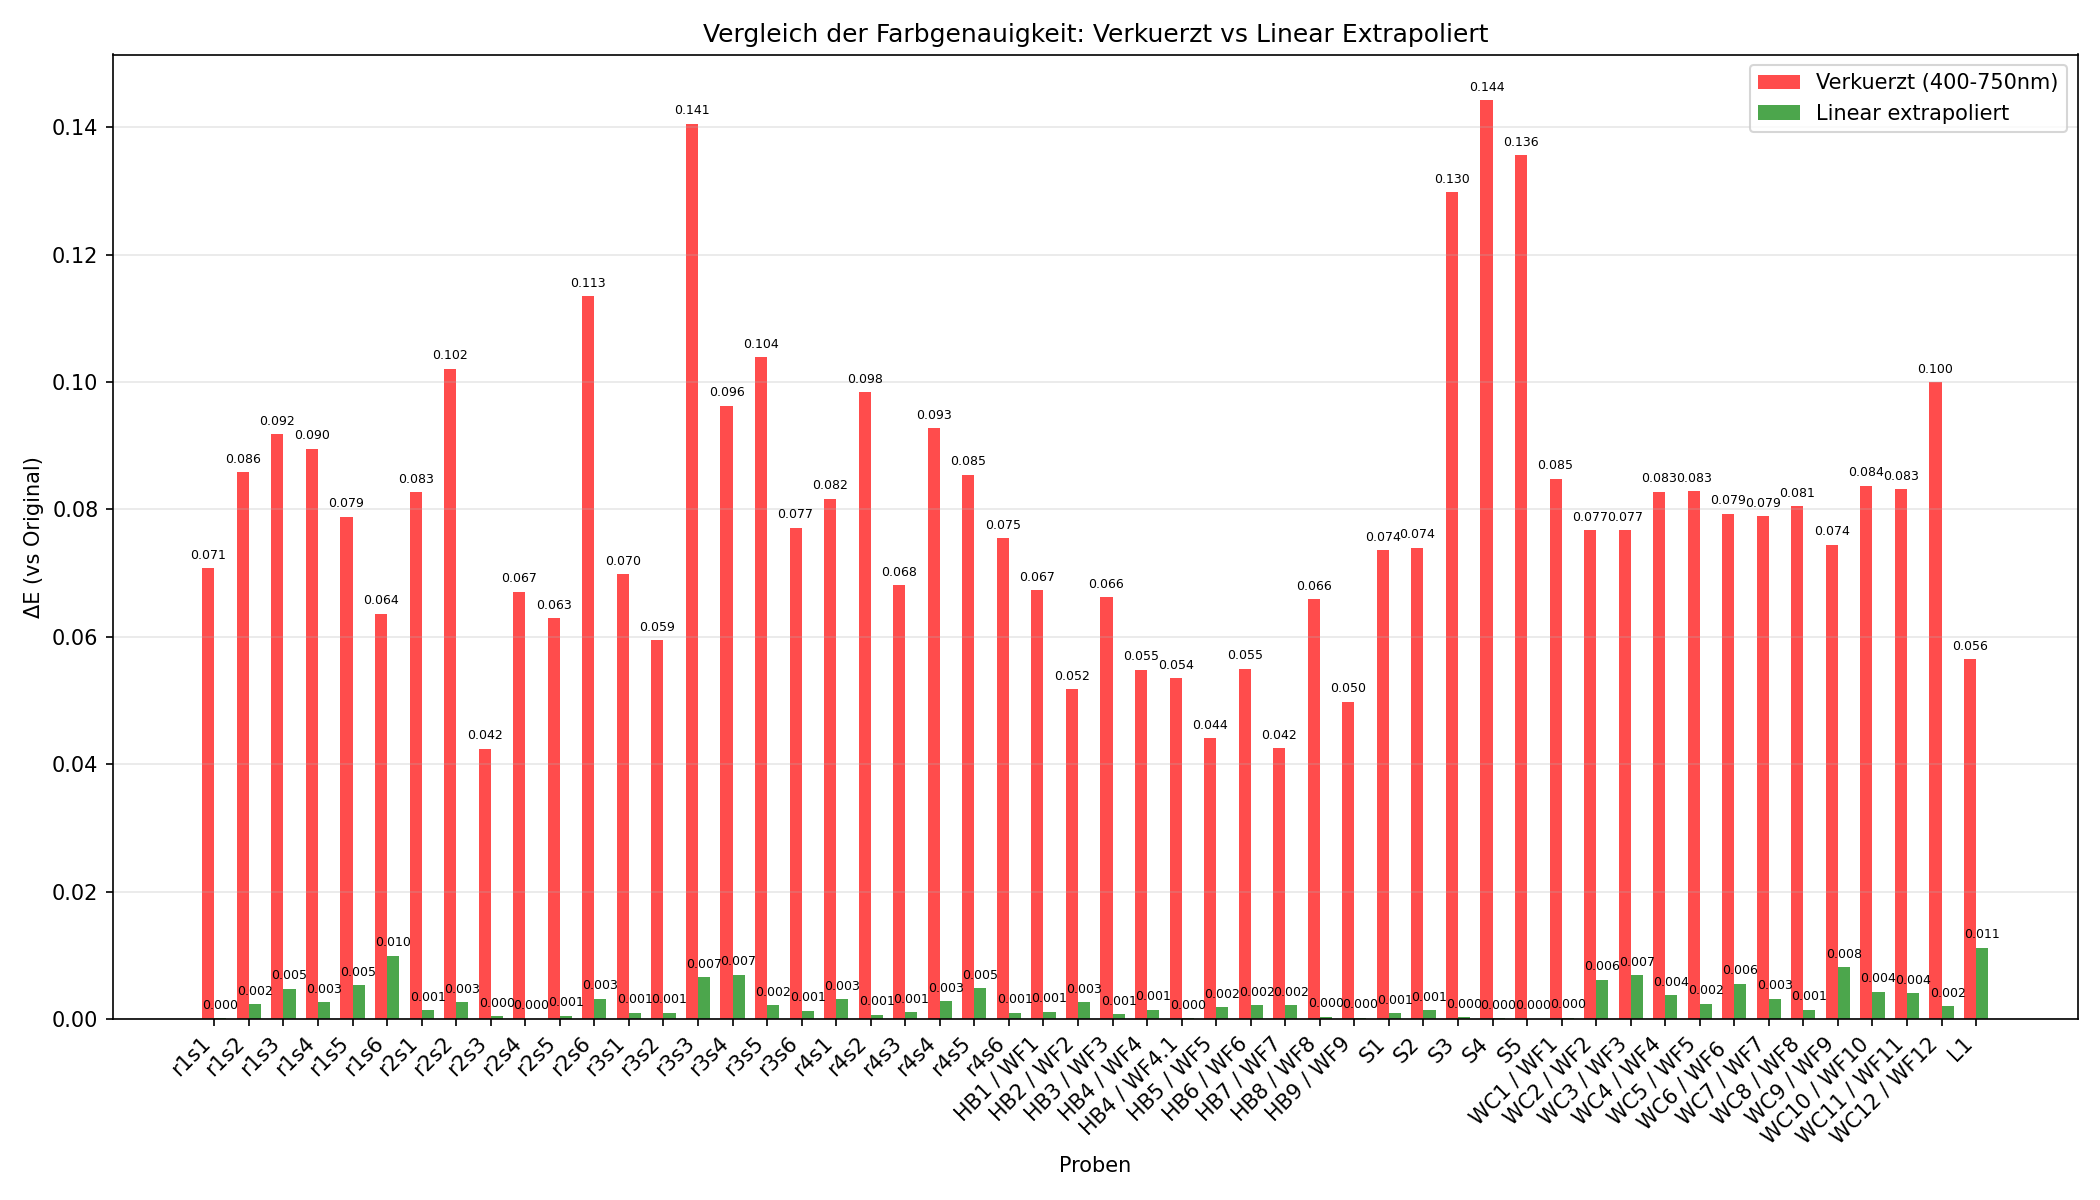
\includegraphics[width=0.9\textwidth]{./figures/delta_e_vergleich_alle_proben.png}
    \caption{Vergleich der Farbfehler vor und nach linearer Extrapolation für die 20 Proben mit den größten Delta E Werten}
    \label{fig:extrapolation_comparison}
\end{figure}

\begin{figure}[htbp]
    \centering
    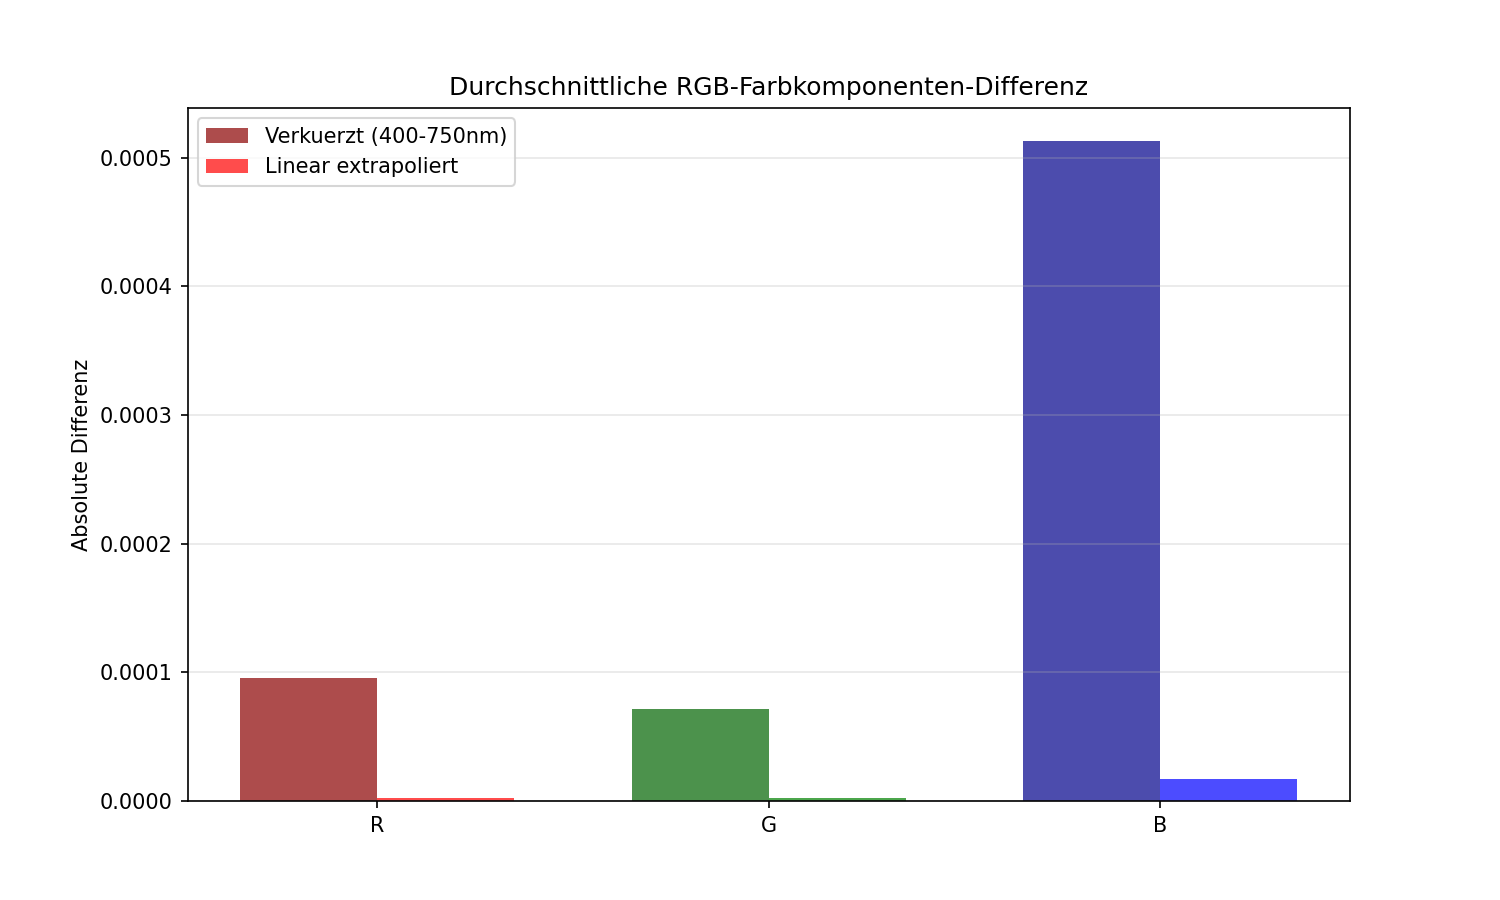
\includegraphics[width=0.8\textwidth]{./figures/rgb_diff_comparison.png}
    \caption{Vergleich der durchschnittlichen RGB-Komponentendifferenzen: verkürzt vs. linear extrapoliert}
    \label{fig:rgb_extrapolation_comparison}
\end{figure}

Die Analyse der RGB-Komponenten nach Extrapolation (Abbildung \ref{fig:rgb_extrapolation_comparison}) zeigt eine drastische Reduktion der Fehler in allen drei Farbkanälen, wobei die Verbesserung bei der B-Komponente am deutlichsten ausfällt.

\section{Diskussion}

\subsection{Praktische Relevanz der Ergebnisse}

Die durchschnittliche Farbdifferenz von $\Delta E = 0.0798$ bei Verkürzung des Wellenlängenbereichs liegt deutlich unter der allgemein akzeptierten Wahrnehmungsschwelle von $\Delta E = 1.0$. Dies bedeutet:

\begin{itemize}
    \item Für die meisten praktischen Anwendungen ist der verkürzte Wellenlängenbereich (400-750 nm) ausreichend
    \item Die resultierenden Farbunterschiede sind für das menschliche Auge nicht wahrnehmbar
    \item Kostengünstigere Spektrometer mit eingeschränktem Wellenlängenbereich können für viele Anwendungen eingesetzt werden
\end{itemize}

\subsection{Sonderfälle und kritische Proben}

Einige Proben zeigten überdurchschnittlich hohe Farbfehler:
\begin{itemize}
    \item \textbf{S4} ($\Delta E = 0.1442$): Grauton mit ausgeprägter spektraler Struktur in den Randbereichen
    \item \textbf{r3s3} ($\Delta E = 0.1406$): Ähnliche spektrale Charakteristik
    \item \textbf{S5} ($\Delta E = 0.1356$): Weiterer Grauton mit Randbereichseinflüssen
\end{itemize}

Diese Proben profitieren besonders stark von der Extrapolationsmethode.

\subsection{Grenzen der linearen Extrapolation}

Obwohl die lineare Extrapolation in allen untersuchten Fällen zu Verbesserungen führte, sind folgende Einschränkungen zu beachten:

\begin{itemize}
    \item Die Methode setzt relativ glatte spektrale Verläufe in den Randbereichen voraus
    \item Bei Proben mit starken spektralen Strukturen nahe 400 nm oder 750 nm könnte die Approximation ungenau werden
    \item Die Extrapolation basiert auf der Annahme, dass der spektrale Gradient konstant bleibt
\end{itemize}

\section{Schlussfolgerungen und Empfehlungen}

\subsection{Haupterkenntnisse}

\begin{enumerate}
    \item Die Verkürzung des Messbereichs von 380-780 nm auf 400-750 nm führt zu durchschnittlichen Farbfehlern von $\Delta E = 0.0798$, die unter der Wahrnehmungsschwelle liegen
    
    \item Die Hauptursache für Farbfehler ist der Verlust spektraler Information in Bereichen, wo das menschliche Auge zwar wenig empfindlich ist, aber dennoch zur Gesamtfarbwahrnehmung beiträgt
    
    \item Lineare Extrapolation kann die Farbfehler um durchschnittlich 96.6\% reduzieren
    
    \item Graue und neutrale Farbtöne sind tendenziell stärker von Wellenlängenbegrenzungen betroffen als bunte Farben
\end{enumerate}

\subsection{Praktische Empfehlungen}

Basierend auf den Forschungsergebnissen können folgende Empfehlungen ausgesprochen werden:

\textbf{Für Standardanwendungen:}
\begin{itemize}
    \item Ein Messbereich von 400-750 nm ist für die meisten praktischen Anwendungen ausreichend
    \item Die resultierenden Farbfehler sind vernachlässigbar klein
    \item Bei Bedarf kann eine lineare Extrapolation implementiert werden
\end{itemize}

\textbf{Für Präzisionsmessungen:}
\begin{itemize}
    \item Der vollständige Bereich 380-780 nm sollte verwendet werden
    \item Besondere Vorsicht bei neutralen/grauen Proben
    \item Validierung der Extrapolationsmethode für spezifische Anwendungsfälle
\end{itemize}

\textbf{Für Geräteentwicklung:}
\begin{itemize}
    \item Integration der linearen Extrapolation als Standardfunktion
    \item Benutzerhinweise bei Messungen nahe der Wellenlängengrenzen
    \item Option zur Anzeige der extrapolierten Bereiche
\end{itemize}

\section{Ausblick}

Die vorliegende Untersuchung eröffnet mehrere Ansatzpunkte für weiterführende Forschung:

\begin{itemize}
    \item \textbf{Erweiterte Extrapolationsmethoden}: Untersuchung von polynomialen oder spline-basierten Extrapolationsverfahren
    
    \item \textbf{Materialspezifische Analyse}: Systematische Untersuchung verschiedener Materialklassen (Textilien, Lacke, Naturmaterialien)
    
    \item \textbf{Dynamische Wellenlängenbereiche}: Adaptive Anpassung des Messbereichs basierend auf der spektralen Charakteristik der Probe
    
    \item \textbf{Maschinelles Lernen}: Entwicklung von KI-basierten Vorhersagemodellen für die spektralen Randbereiche
\end{itemize}

Die Ergebnisse dieser Forschung tragen dazu bei, die praktische Anwendbarkeit spektraler Messgeräte mit eingeschränktem Wellenlängenbereich besser einschätzen zu können und bieten konkrete Lösungsansätze zur Kompensation der entstehenden Messfehler.
